Our muon tracker is currently producing experimental results, but we have no way of confirming their validity. As such, we propose using CERN’s high-energy Proton Synchrotron as a source of a controlled muon beam and use this experiment to compare our detector tracking results with the known trajectory of the Proton Synchrotron muon beam.

The evaluation of XY translational accuracy will be assessed by aiming the detector’s Z axis toward the beamline and iterating through different XY positions; the evaluation of XYZ rotational accuracy will be done by iterating through diverse altitude and azimuth angles. As the position is encoded to an $8 \times 8$ grid, a minimum of 64 different translations and 64 rotations will confirm the correct triggering of all SiPMs and the faithfulness of the trajectory volume computation with the actual trajectories.
\begin{figure} [h]
    \centering
    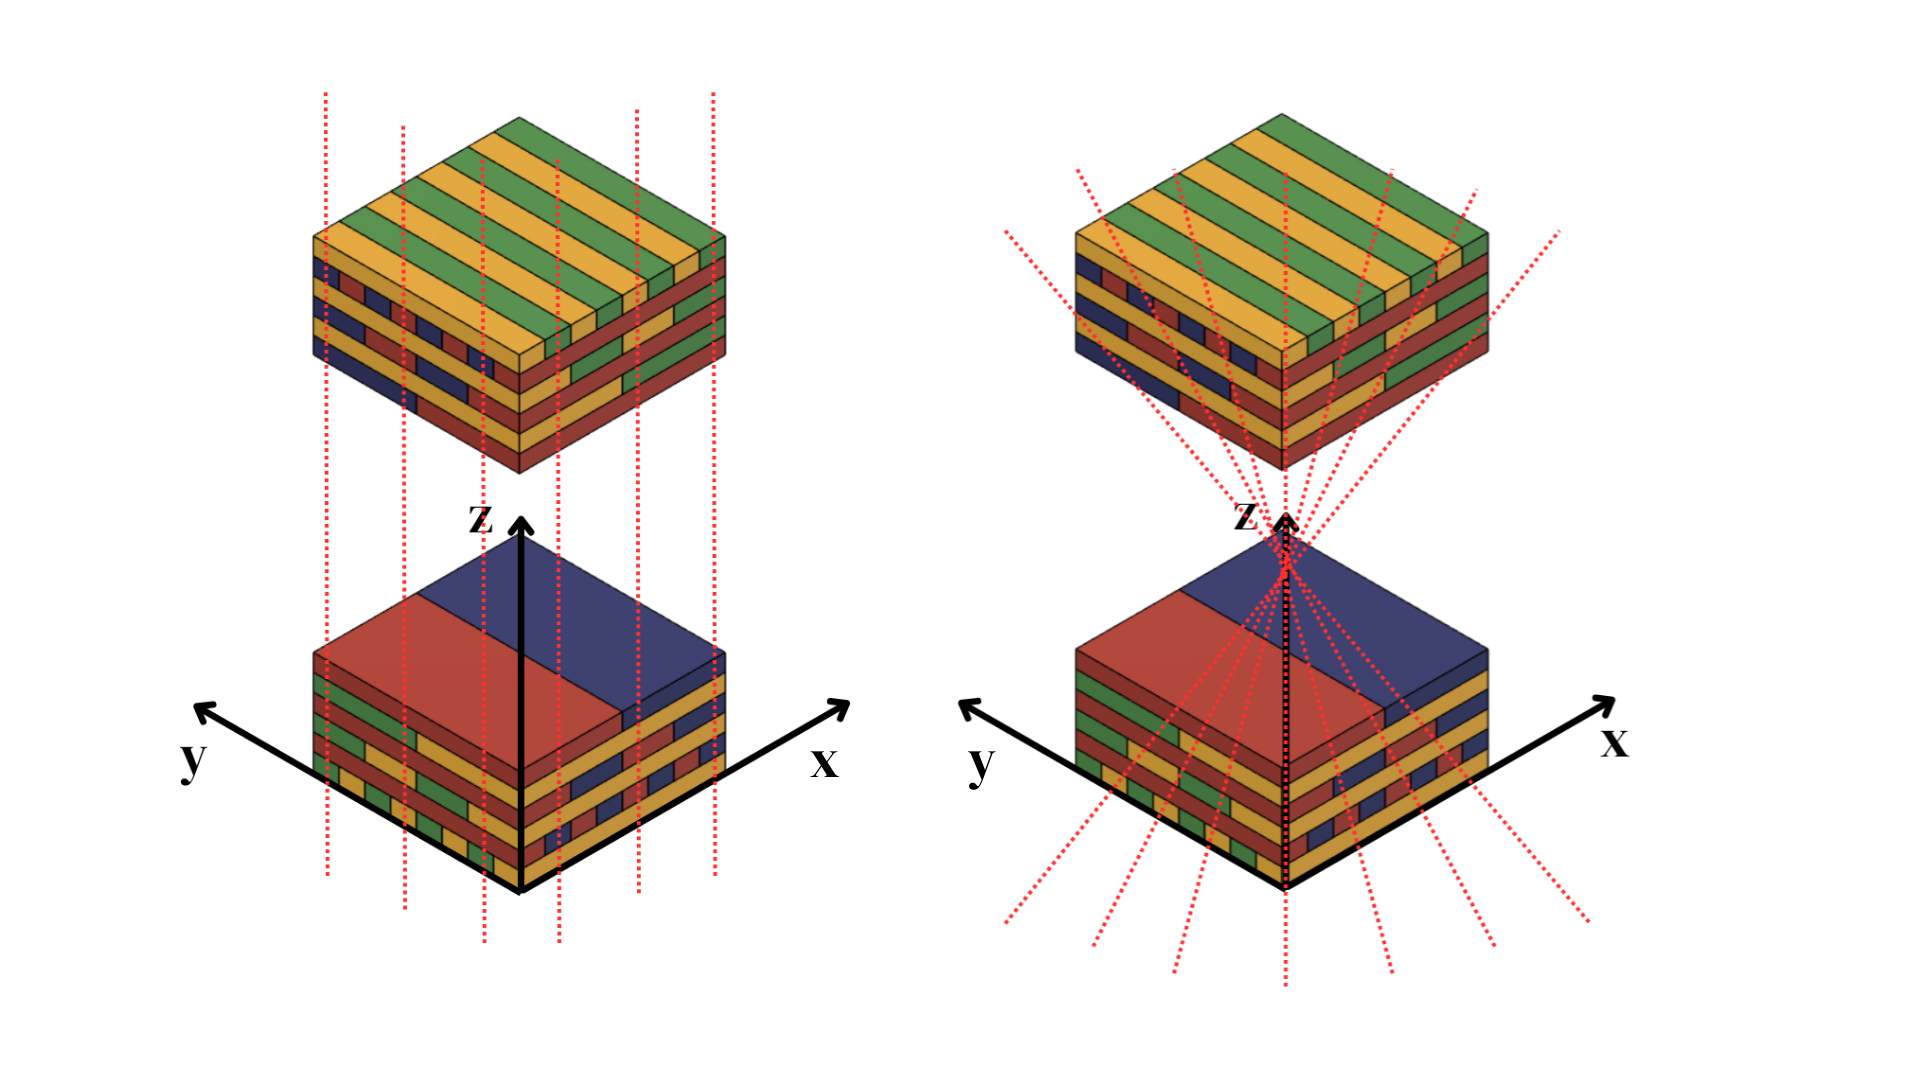
\includegraphics[scale=0.2]{figures/proposed test.png}
    \caption{Experimental proposal axes reference frame. \textbf{Left:} Example XY translational testing beamlines. \textbf{Right:} Example XYZ rotational testing beamlines.}
    \label{proposed tests}
\end{figure}

\begin{figure} [h]
    \centering
    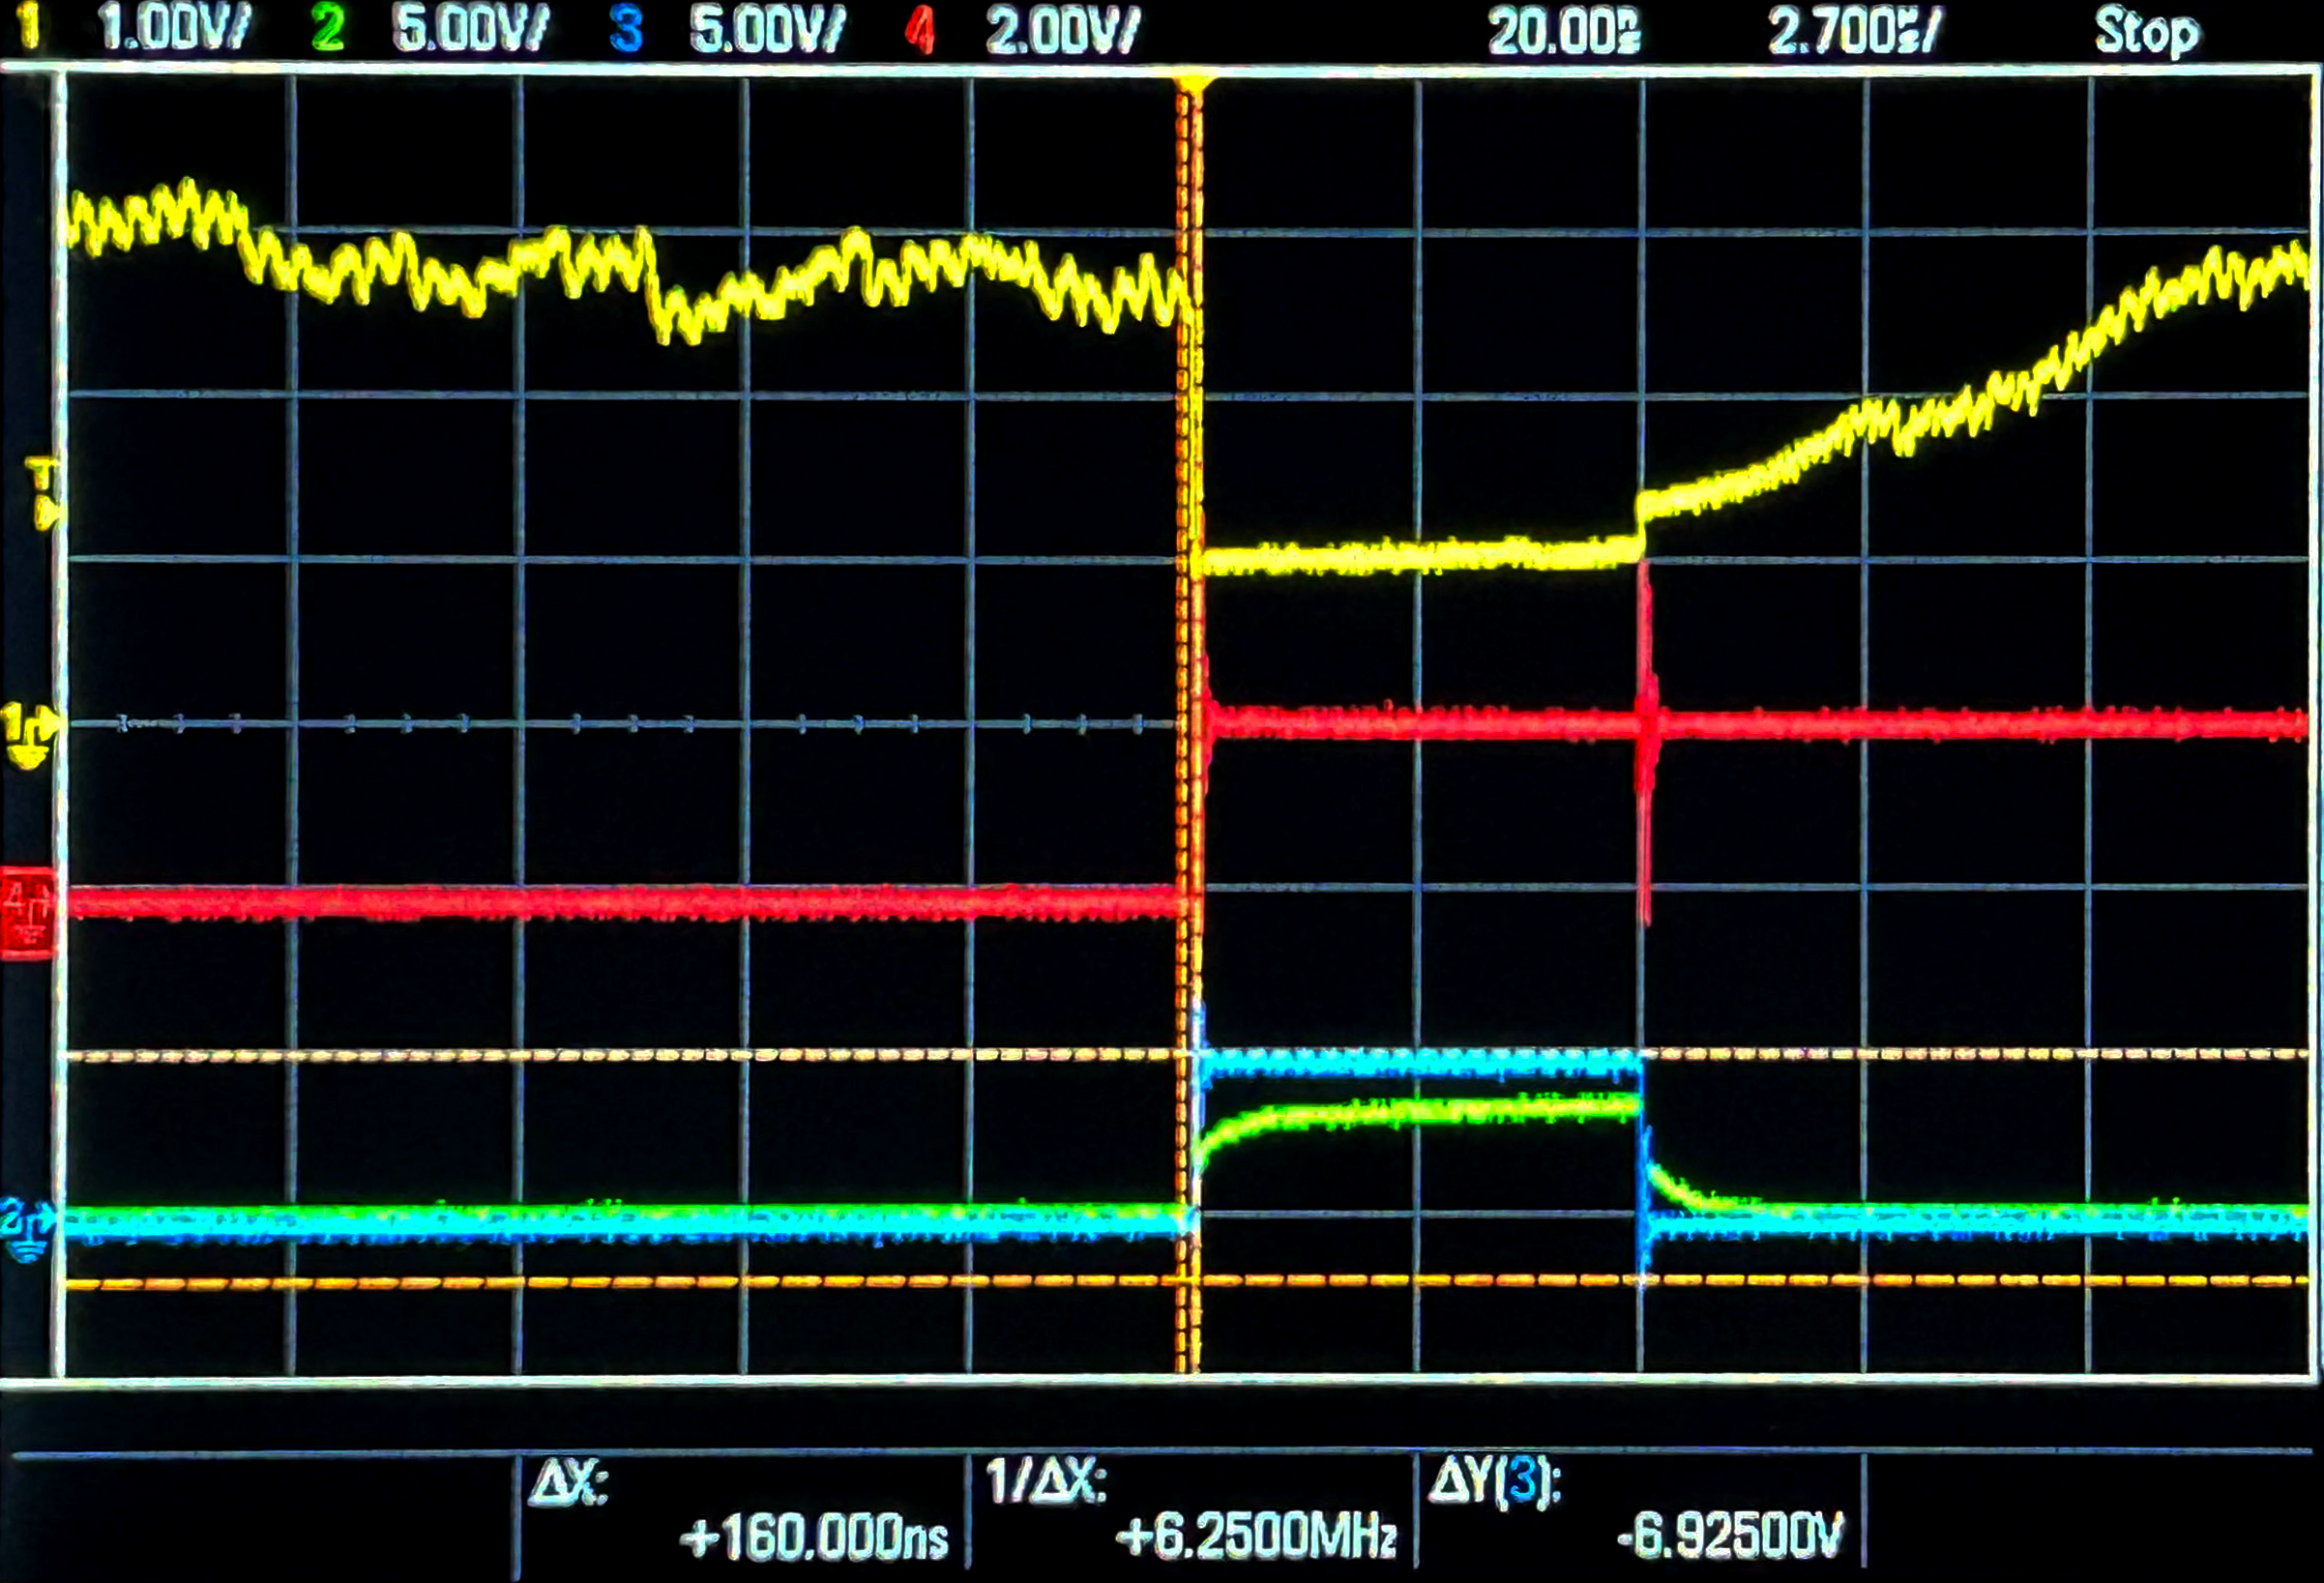
\includegraphics[width=0.58\linewidth]{figures/digitizer all.png}
    \caption{Digitizer circuit signals from acquisition hardware. \textbf{Yellow:} analog output from trans-impedance amplifier connected to comparator inverting input. \textbf{Red:} latching FPGA register for acquisition. \textbf{Blue:} comparator output. \textbf{Green:} level-shifted comparator output. Adjustable comparator threshold voltage: 1.133V $\pm$ 0.1\%.}
    \label{digitizer}
\end{figure}